\documentclass{xdyydoc}

\newcommand{\DocDate}{2022-9-18}
\newcommand{\DocVersion}{v0.1.20}
\usepackage{xeCJKfntef, xpinyin}
\usepackage{graphicx}
\usepackage{zhlipsum}
\usepackage{tabularray}
\usepackage{../exam-zh-choices}
\usepackage{../exam-zh-question}
\usepackage{../exam-zh-symbols}
\usepackage{../exam-zh-chinese-english}
\usepackage{../exam-zh-textfigure}

\ExplSyntaxOn
\NewDocumentCommand \examsetup { m }
  { \keys_set:nn { exam-zh } {#1} }
\ExplSyntaxOff
% \usepackage[
%   backend = biber,
%   style = gb7714-2015
% ]{biblatex}
% \addbibresource{exam-zh.bib}
\graphicspath{{figures}}

\hypersetup{
  pdftitle  = {exam-zh: 高考试卷 LaTeX 模板},
  pdfauthor = {夏康玮}
}
% 全角标点放在引号中,需要改成半角式,否则间距过大,不好看
\def\FSID{“{\xeCJKsetup{PunctStyle=banjiao}。}”} % U+3002
\def\FSFW{“{\xeCJKsetup{PunctStyle=banjiao}.}”} % U+FF0E
\def\COFW{“{\xeCJKsetup{PunctStyle=banjiao}:}”} % U+FF1A
\def\SCFW{“{\xeCJKsetup{PunctStyle=banjiao};}”} % U+FF1B


\title{\textcolor{MaterialIndigo800}{%
  \textbf{exam-zh: 高考试卷 \LaTeX \xpinyin[font=\sffamily,format=\color{MaterialIndigo800}]{模}{mu2}板}}}
\author{李泽平,夏康玮,郭李军}
\date{\DocDate\quad \DocVersion%
  \thanks{%
    \url{https://gitee.com/xkwxdyy/exam-zh}
  }
}

\ExplSyntaxOn
\NewDocumentCommand { \scoringbox } { s }
  {
    \IfBooleanTF {#1}
      { \__examzh_scoringbox_onecolumn: }
      { \__examzh_scoringbox_twocolumn: }
  }
\cs_new_protected:Nn \__examzh_scoringbox_twocolumn:
  {
    \begin{tabular}{|c|c|}
      \hline 
      得分 & \rule{3em}{0pt}\rule[-0.7em]{0pt}{2em} \\\hline
      阅卷人 & \rule{3em}{0pt}\rule[-0.7em]{0pt}{2em} \\\hline
    \end{tabular}
  }
\cs_new_protected:Nn \__examzh_scoringbox_onecolumn:
  {
    \begin{tabular}{|c|}
      \hline 
      得分\rule[-0.7em]{0pt}{2em} \\\hline
      \rule[-0.7em]{0pt}{2em} \\\hline
    \end{tabular}
  }
\ExplSyntaxOff

\AddToHook{env/latexexample/after}
  {%
    \examsetup{
      question/index=1
    }
  }
\usepackage{amssymb}

\begin{document}

% 封面的页边距

\newgeometry{
  left   = 2.2 in,
  right  = 1.25 in,
  top    = 1.25 in,
  bottom = 1.00 in
}

\maketitle

% !TeX root = ../exam-zh-doc.tex

\begin{abstract}
  本项目提供了一个中国高考试卷样式的 \LaTeX 模板,旨在帮助中小学教师更方便地使用 \LaTeX。模板具有以下特性:
  
  \begin{enumerate}
    \item 样式与内容尽可能分离;
    \item 选择题选项可以自动排版成合适的列数;
    \item 通过用户接口可以方便更改密封线样式;
    \item 在 Windows, macOS 和 Linux 跨平台编译。
  \end{enumerate}
\end{abstract}


\begin{tikzpicture}[remember picture, overlay]
  \node[opacity = 0.1,rotate = 30] at ([shift={(0,0)}]current page text area.center){
    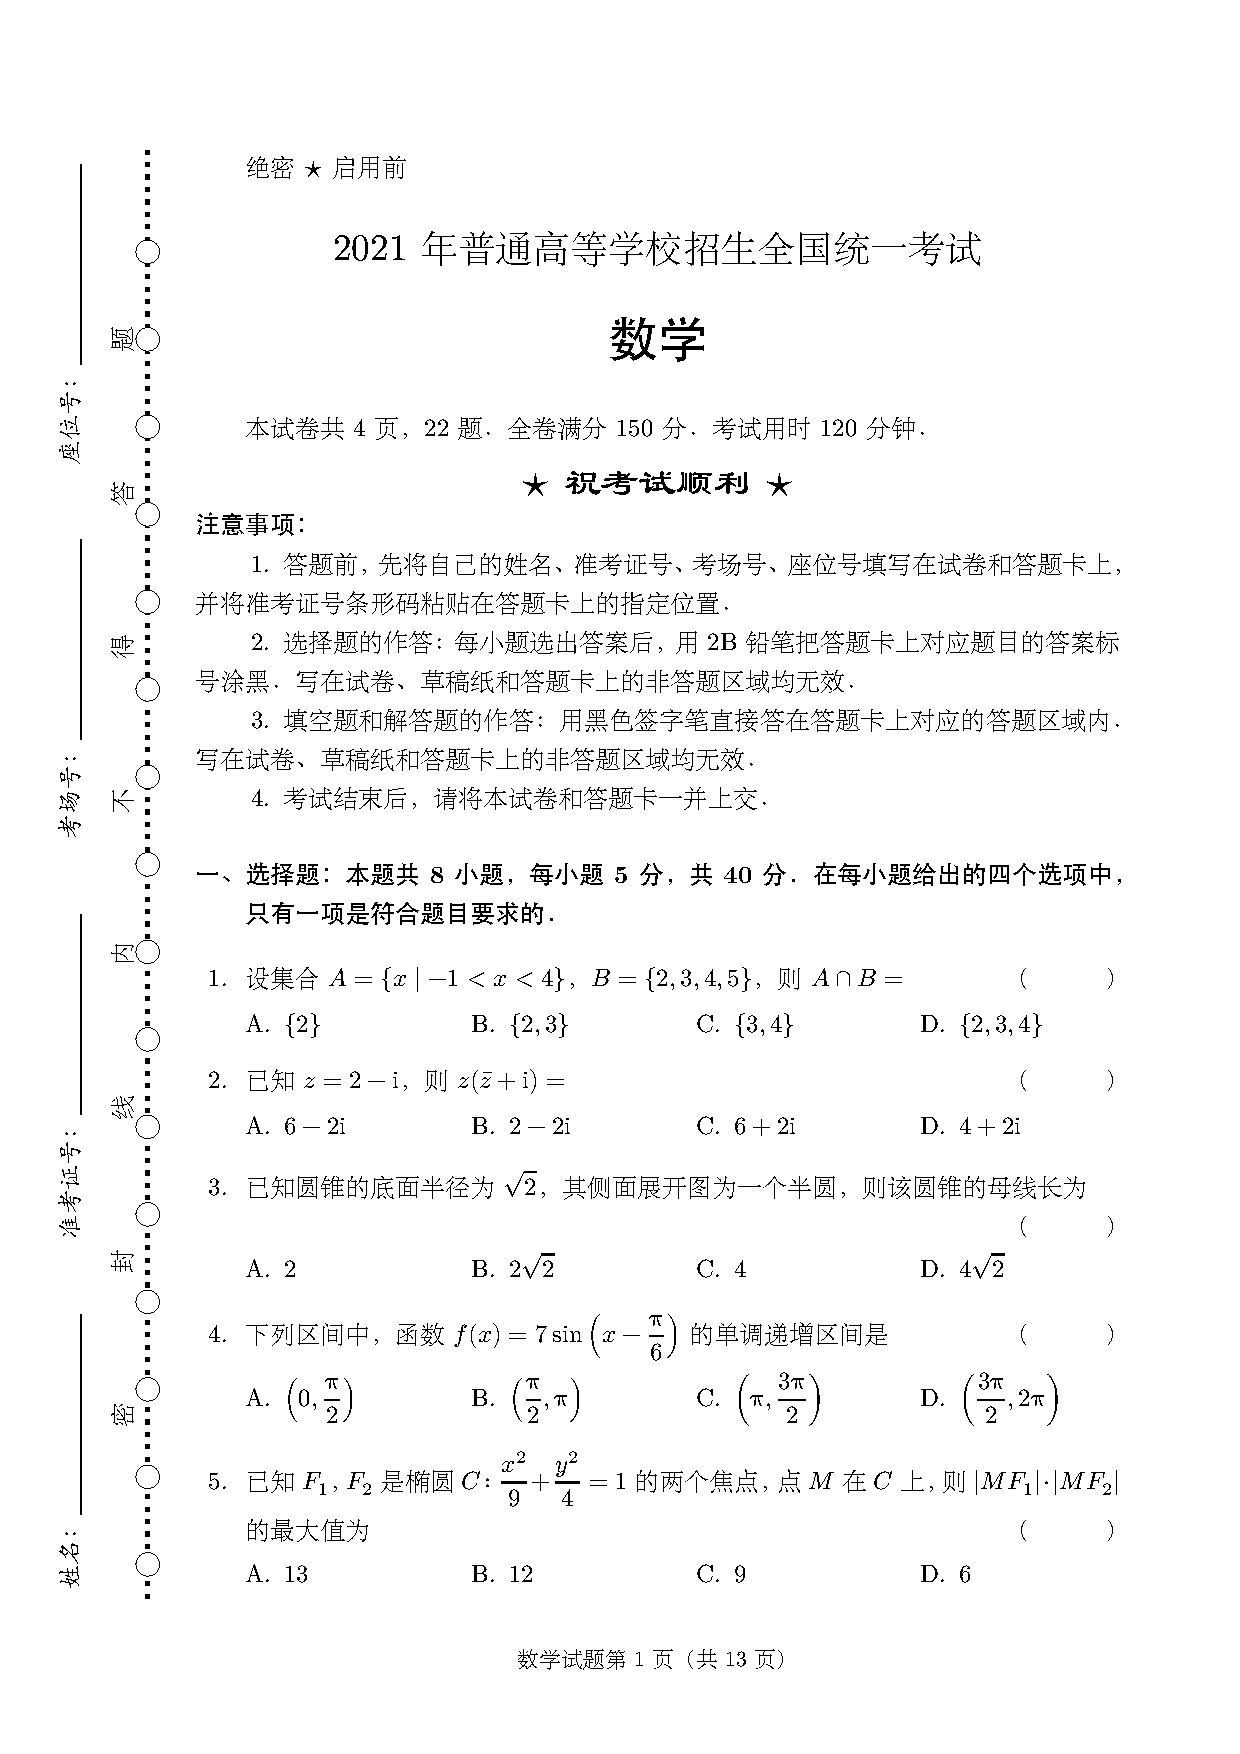
\includegraphics[width=23cm]{firstpage.pdf}
  };
\end{tikzpicture}
\thispagestyle{plain}
\clearpage


% 用户手册的页边距

\newgeometry{
  left   = 1.75 in,
  right  = 0.80 in,
  top    = 1.25 in,
  bottom = 1.00 in
}

\tableofcontents


% 介绍
\chapter{引~~言}\label{chap:introduction}

\section{编写说明}
\upcite{Arteaga-Falconi:ITIM:2016}\upcite{Barni:ITIFS:2011}
\upcite{Dautov:IJBHI:2016,Hartley:ITITB:2012,Hu:ITITB:2007}
研究生学位论文是作者攻读研究生期间研究成果的总结,是衡量作者是否达到研究生水平的重要依据。同时,研究生学位论文也是反映最高层次学历教育水平的学术作品,学校图书馆、中国学术期刊网等将作为学术资料长期保存,供同行学者、后续研究者查阅和参考。因此,要求学位论文文字正确,语言通顺,数据可靠,表述清晰,图、表、公式、单位等符合规范要求。同时,作为湘潭大学的研究生学位论文,在符合国家关于学位论文编写规范要求的基础上,应有统一的格式。

为此,研究生处依据中华人民共和国国家标准《科学技术报告、学位论文和学术论文的编写格式》(GB/T 7713—1987)、《文后参考文献著录规则》(GB/T 7714—2005),参照《清华大学博士学位论文写作指南》,编写了《湘潭大学研究生学位论文写作指南》,供研究生撰写学位论文时参考。

本《写作指南》只是一个指导性的文件。相关学科有特殊要求的,由学位点在本《写作指南》的基础上编写出相应学科的《写作指南》,报校学位办备案后执行。

\section{学位论文的基本要求}
国家标准《科学技术报告、学位论文和学术论文的编写格式》(GB7713—1987)中指出:学位论文是表明作者从事科学研究取得创造性的结果或有了新的见解,并以此为内容撰写而成、作为提出申请授予相应的学位时评审用的学术论文[1]。

研究生学位论文是研究生在导师指导下独立完成的、系统完整的学术研究工作的总结,论文应体现出研究生在所属学科领域做出的创造性学术成果,应能反映出研究生已经掌握了相应学位层次要求的基础理论和专门知识,并具备了独立从事学术研究工作的能力。

\section{撰写学位论文的语言及文字}
研究生学位论文要求用汉语书写,所用汉字须符合国家语言工作委员会、中华人民共和国新闻出版署联合发布的《现代汉语通用字表》[2]。专用名词、术语可采用国际通用的代号,量及其单位所使用的符号应符合国家标准《国际单位制及其应用》(GB3100—1993)[3]、《有关量、单位和符号的一般原则》(GB3101—1993)[4]的规定。图、表中的图题、坐标轴、图例、表头等描述性的词组或语句须使用汉语,专用名词术语、物理量及其单位可使用符合规范要求的符号。

外国人来华留学生可以用英文撰写学位论文,但须采用中文封面,且应有不少于6000字的详细中文摘要。

\section{主要内容}
本《写作指南》包括以下四方面内容:第一部分引言,阐述编写本《写作指南》的目的,以及按规范撰写论文的重要性;第二部分,湘潭大学研究生学位论文的基本格式要求,包括论文由哪些部分组成,排列顺序、装订方式、页面设置等具体格式要求;第三部分,参考文献著录规则及注意事项;第四部分,研究生学位论文中一些主要部分的写作方法和要求。此外,在附录中提供了部分模板样式(中文封面、英文封面及学位论文原创性声明与版权使用授权书),供研究生撰写论文时参考。 
% 安装
% !TeX root = ../exam-zh-doc.tex

\section{安装与更新}


\subsection{标准安装}

目前 \cls{exam-zh} 已经上传 CTAN,您可以使用宏包管理器安装 \cls{exam-zh}。
例如在 \TeXLive{} 中,执行(可能需要管理员权限)
\begin{shellcode}[morekeywords={tlmgr,install}]
  tlmgr install exam-zh
\end{shellcode}
即可完成安装。

在 \TeXLive{} 和 \MiKTeX{} 中,您还可以通过图形界面进行安装,
此处不再赘述。


\subsection{手动安装}

您也可以通过访问 gitee 项目主页的方式获取最新版本的 \cls{exam-zh}(通常情况下,gitee 的版本会大于等于CTAN 的版本(因为 CTAN 从上传到审核到用户可以下载需要一天左右))。主要以「下载发行版」的方式获取最新版本的 \cls{exam-zh}:

\begin{enumerate}
  \item 进入项目主页(\href{https://gitee.com/xkwxdyy/exam-zh}{gitee 项目主页} (界面见图~\ref{figure:gitee项目主页} )
  \item 在右侧一列有“发行版”(gitee),并且有一个标签图标并有“vx.x.x - 20xx-xx-xx”字样,表示最新的发行版版本和发布时间,点击即可查看相关信息(如果想查看历史所有发行版信息,可以点击“发行版”右侧的“全部”(gitee))。
  
    发行版中一般由以下信息构成(\href{https://gitee.com/xkwxdyy/exam-zh/releases}{gitee 发行版} 界面见图~\ref{figure:gitee发行版})
      \begin{itemize}
        \item 更新文件的特别说明。如果没有,则表明此次更新只需要更新 \file{exam-zh.cls} 文件至最新\footnote{“更新 \meta{文件} 至最新”目前表示在发行版中下载最新版本的模板,并用其中所需要更新的 \meta{文件} 去替换本地的旧 \meta{文件}} 即可
        \item 更新日志。 主要为此次发行版与上次发行版的不同,一般为“Added”、“Changed”、“Fixed”等信息
        \item 模版及用户手册下载链接(“下载”部分)。一般用户只需要点击 \file{exam-zh-vx.x.x.zip} 进行模版下载即可,而下面的 \file{Source code} 为项目的整个源码,包括手册的源码,测试文件等,如果感兴趣的用户可以下载进行查看(当然,如果会使用 \cmd{git} 的用户也可以将整个 \cls{exam-zh} 项目 \cmd{clone} 下来查看)
      \end{itemize}
  \item 点击 \file{exam-zh-vx.x.x.zip} 进行下载,在本地解压即可
\end{enumerate}


\begin{figure}[htbp]
  \centering
  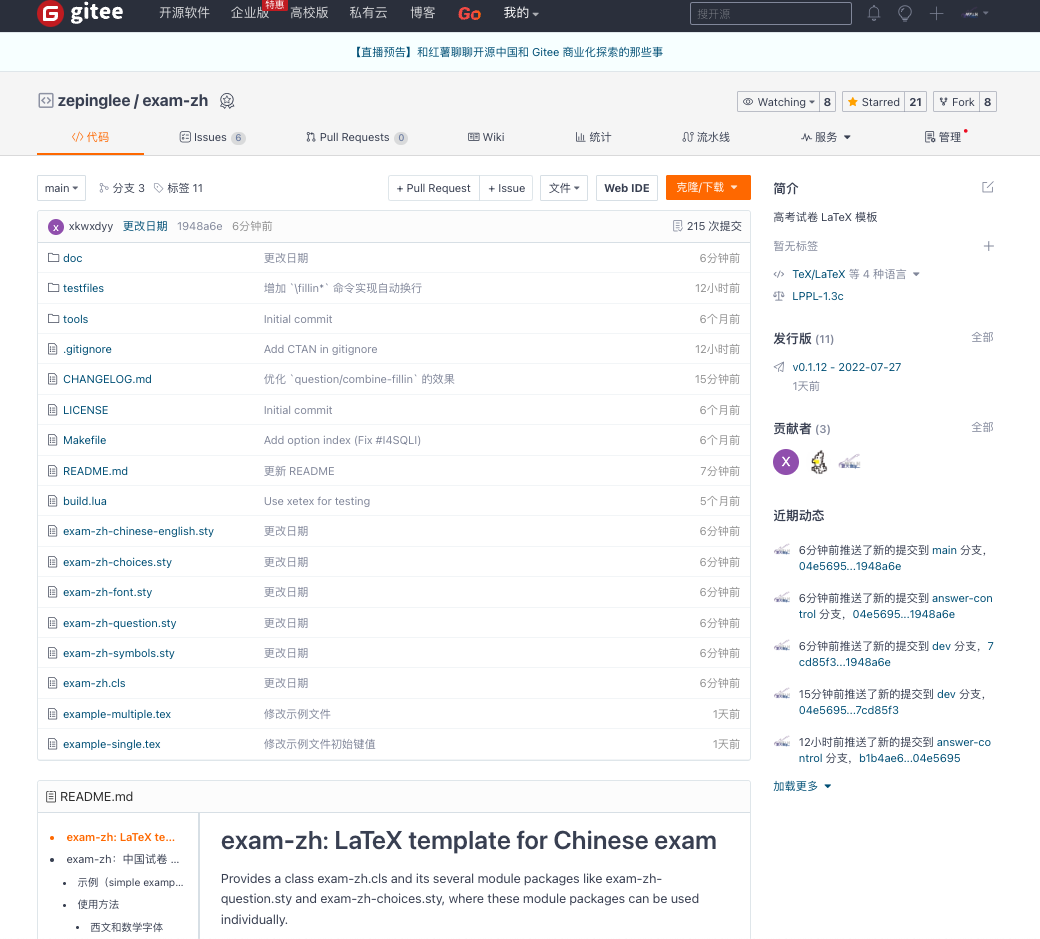
\includegraphics[width = \textwidth]{gitee-main.png}
  \caption{gitee 项目主页}
  \label{figure:gitee项目主页}
\end{figure}


\begin{figure}[htbp]
  \centering
  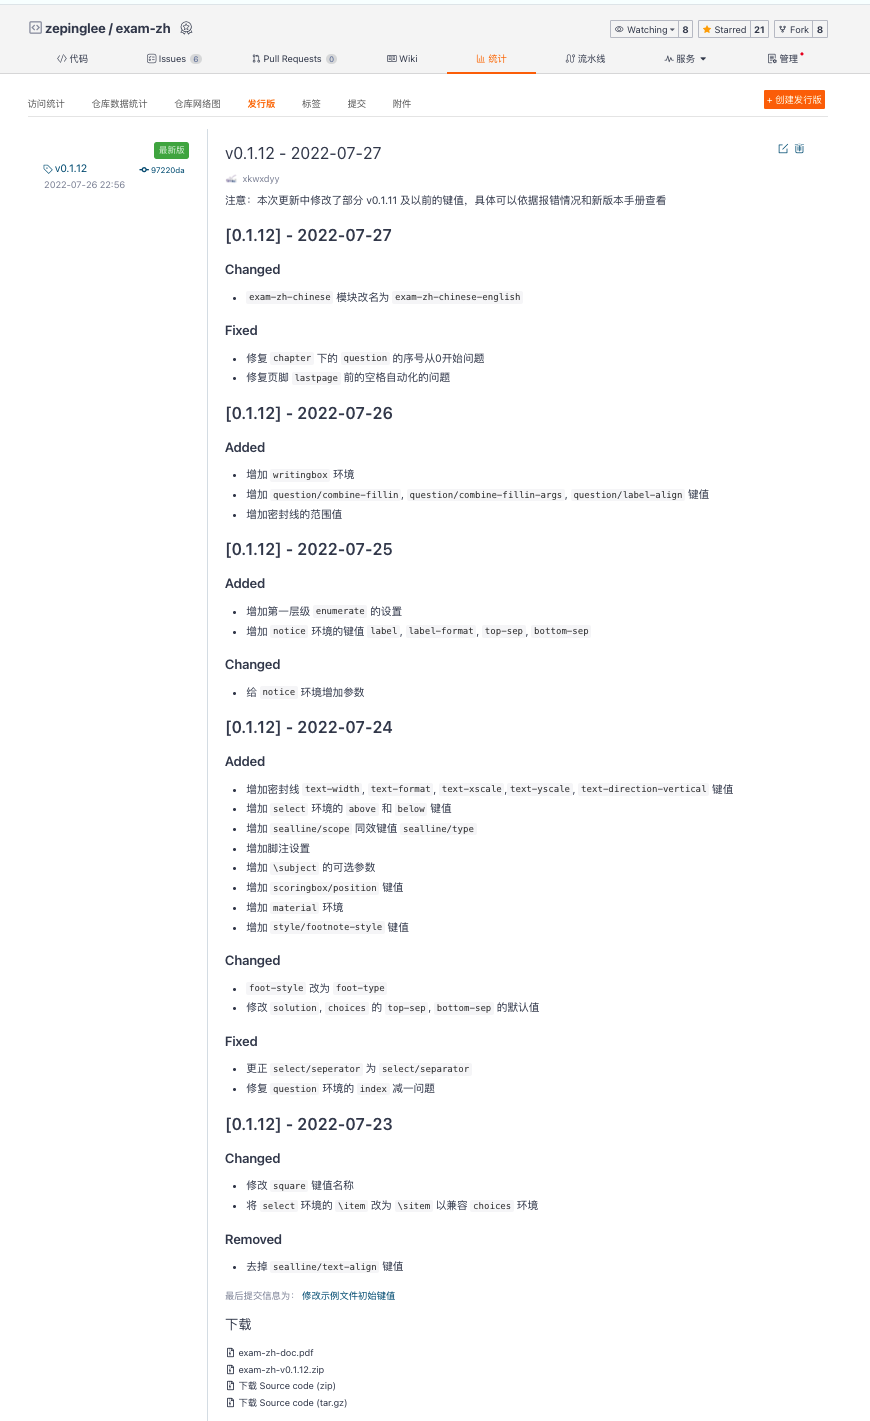
\includegraphics[width = 0.8\textwidth]{gitee-release.png}
  \caption{gitee 发行版}
  \label{figure:gitee发行版}
\end{figure}



\subsection{模板组成}

本模板主要包含核心文档类、参考文献格式文件以及用户文档等几个部分,
其具体组成见表~\ref{tab:exam-zh-main-components}。

\begin{table}[htbp]
  \caption{\cls{exam-zh} 的主要组成部分}
  \label{tab:exam-zh-main-components}
  \centering
  \small
  \begin{tblr}{
    hline{1, 2, Z} = {1pt},
    width = \textwidth,
    colspec = {X[3,l]X[5.5,l]},
    rows = {m}
  }
    \textbf{文件} & \textbf{功能说明} \\
    \file{exam-zh-doc.pdf}            & 用户手册(本文档) \\
    \file{example-single.tex}、\file{example-multiple.tex}            & 模板的主文件(同时也是示例文件),可据此为基础完成试卷编写 \\
    \file{exam-zh.cls}            & 模板文档类 \\
    \file{exam-zh-choices.sty}    & 模版的选择题模块宏包\\
    \file{exam-zh-question.sty}   & 模版的题干模块宏包\\
    \file{exam-zh-font.sty}       & 模版的字体模块宏包\\
    \file{exam-zh-symbols.sty}    & 模版的符号模块宏包\\
    \file{exam-zh-chinese-english.sty}    & 模版的语文英语模块宏包\\
    \file{exam-zh-textfigure.sty}    & 模版的图文排版模块宏包\\
    \file{README.md}              & 简要自述 \\
    \file{CHANGELOG.md}           & 模板更新日志 \\
    \file{LICENSE}                & 模版发布许可证
  \end{tblr}
\end{table}

% \begin{table}[htbp]
%   \caption{\cls{exam-zh} 各目录的组成部分}
%   \label{tab:exam-zh-sub-components}
%   \centering
%   \small
%   \begin{tblr}{
%     hline{4,5,8,11,13} = {solid},
%     hline{1, 2, Z} = {1pt},
%     width = \textwidth,
%     colspec = {X[1,l]X[3,l]X[3,l]},
%     rows = {m},
%     cell{2}{1} = {r=2}{m},
%     cell{5}{1} = {r=3}{m},
%     cell{8}{1} = {r=3}{m},
%     cell{11}{1} = {r=2}{m},
%   }
%     \textbf{子目录} & \textbf{子目录中的文件} & \textbf{功能说明} \\
%     front & \file{abstract.tex}            & 中英文摘要 \\
%     front & \file{notation.tex}            & 符号表 \\
%     body  & \file{chapter<number>.tex}     & 正文的分文件 \\
%     back  & \file{acknowledgements.tex}    & 致谢 \\
%     back  & \file{appendix.tex}            & 附录 \\
%     back  & \file{publications.tex}        & 攻读学位期间取得的研究成果(博士)\\
%     logo  & \file{ccnulogo.png}            & “华中师范大学”字样 logo \\
%     logo  & \file{masterlogo.png}          & 硕士学位论文页眉 logo \\
%     logo  & \file{doctorlogo.png}          & 博士学位论文页眉 logo \\
%     copyright  & \file{Originality_Copyright.pdf}  & 本科学位论文原创性声明和使用授权说明 \\
%     copyright  & \file{Originality_Copyright_master_doctor.pdf}  & 硕博学位论文原创性声明和使用授权说明\\
%     figures & & 用户放置图片的目录\\
%   \end{tblr}
% \end{table}

% \clearpage
% 使用
%%
%% usage.tex
%% Copyright 2011 Zoran Filipovi\'{c}
%
% This work may be distributed and/or modified under the
% conditions of the LaTeX Project Public License, either version 1.3
% of this license or (at your option) any later version.
% The latest version of this license is in
% http://www.latex-project.org/lppl.txt
% and version 1.3 or later is part of all distributions of LaTeX
% version 2005/12/01 or later.
%
% This work has the LPPL maintenance status `maintained'.
%
% The Current Maintainer of this work is Zoran Filipovi\'{c}
%
%%
\documentclass[12pt]{article}
\usepackage[T1]{fontenc}
\usepackage[latin1]{inputenc}

\title{Serbian cyrillic support}
\author{Zoran Filipovi\'{c}}

\begin{document}
\maketitle
\abstract{This document present in which way how you use 
          \verb|serbian-def-cyr| package.}


\section{Introdaction}

This package present support for serbian language in cyrillic scripts in 
way which is macro and definitions, such like \verb|abrstract|, \verb|title|, 
\verb|chapter| etc., present in cyrillic scripts. Translations for this macro 
exist in \verb|babel| package for serbian language in latin script. Package 
working in T2A font encoding, and code page is cp 1251.  

\section{How to use this package?}

Just put a  line \verb|\usepackage{serbian-def-cyr}| in preambula for 
you document. If you use \verb|WinShell| us \LaTeX\
editor you must in \verb|Options|, \verb|Fonts|, \verb|Script| set on
\verb|Cyrillic|, and coding is \verb|Standard|. Also, set the keyboard on
serbian language in cyrillic scripts. 


\end{document}


% 宏包依赖情况
% !TeX root = ../exam-zh-doc.tex

\section{宏包依赖情况}

\begin{itemize}
  \item \pkg{expl3}:提供 \LaTeX3 环境
  \item \pkg{xparse}:自定义命令环境
  \item \pkg{filehook}:给宏包打补丁
  \item \cls{ctexbook}:\cls{exam-zh} 基于的文档类
  \item \pkg{etoolbox}:补丁
  \item \pkg{geometry}:页面设置
  \item \pkg{fontspec}:字体设置
  \item \pkg{xeCJK}、\pkg{xeCJKfntef}:中文相关
  \item \pkg{fancyhdr}:页眉页脚
  \item \pkg{lastpage}:总页数
  \item \pkg{amsmath}、\pkg{unicode-math}:数学类宏包
  \item \pkg{amsthm}:提供 \tn{qed} 相关
  \item \pkg{enumitem}:列表
  \item \pkg{tikz}、\pkg{tikzpagenodes}: \TikZ
  \item \pkg{hyperref}:超链接
  \item \pkg{zref}、\pkg{zref-savepos}:记录位置。
  \item \pkg{ulem}:下划线
  \item \pkg{tcolorbox}:彩框
  \item \pkg{varwidth}:“弹性”的 \env{minipage}
\end{itemize}


\file{exam-zh-textfigure.sty} 的宏包依赖:

\begin{itemize}
  \item \pkg{wrapstuff}:图文混排
  \item \pkg{tabularray}:表格
  \item \pkg{varwidth}:“弹性”的 \env{minipage}
  \item \pkg{graphicx}:插图
\end{itemize}
% 主要更新
% !TeX root = ../exam-zh-doc.tex

\section{主要更新}

\begin{itemize}
  \item 2022.2 开发基本框架和主要功能(题干、选择题)
  \item 2022.4 开发字体模块
  \item 2022.6 开发密封线、草稿纸、评分框
  \item 2022.7 增加语文英语题型
\end{itemize}

% 参与开发
% !TeX root = ../exam-zh-doc.tex

\section{参与开发}

\begin{itemize}
  \item 如果您有任何改进意见或者功能需求,欢迎前往 \href{https://gitee.com/xkwxdyy/exam-zh/issues}{gitee 仓库 issues} 提交 issue
  \item 欢迎 \cmd{fork} 本项目,提 \cmd{pr} 的形式参与开发
  \item 建议阅读 \href{https://zhuanlan.zhihu.com/typography-and-latex/}{muzimuzhi} 写的 \href{https://gitee.com/ustctug/ustcthesis/wiki/%E5%8F%82%E4%B8%8E%E5%BC%80%E5%8F%91}{参与开发}
  \item 参考阅读
    \begin{itemize}
      \item \href{https://www.zhihu.com/question/27017364/answer/34932199}{知乎:开发一个 LaTeX 宏包需要多少知识?}
      \item \href{https://zhuanlan.zhihu.com/p/19669122}{The TeXbook 导读:从那头(多图杀猫的)狮子说起}
    \end{itemize}
\end{itemize}


% 关于作者
% !TeX root = ../exam-zh-doc.tex

\section{关于模版作者和维护者}

\href{https://github.com/zepinglee}{zepinglee} 开发了模版前期的大框架和主要功能(\file{exam-zh-choices.sty}、\file{exam-zh-question.sty}、\file{exam-zh-font.sty} 等)。

\href{https://github.com/xkwxdyy}{xkwxdyy} 和 \href{https://github.com/ljguo1020}{ljguo} 为模版的后期维护者。

非常感谢 \href{https://github.com/syvshc}{syvshc} 在开发中提供的帮助!



\section{\cls{exam-zh}:TODO}

\begin{itemize}
  \item 增加试卷范例(语文,英语)
  \item 答案控制
    \begin{itemize}
      \item 选择题
        \begin{itemize}
          \item 题目下方
          \item 括号内
          \item 最后:列表形式、表格形式
        \end{itemize}
      \item 填空题
        \begin{itemize}
          \item 题目下方
          \item 划线内
          \item 最后
        \end{itemize}
      \item 解答题
        \begin{itemize}
          \item 题目下方
          \item 移动到最后
        \end{itemize}
    \end{itemize}
  \item 选择题答案标记
  \item 图文排版(参考 xkwxdyy 的 \pkg{text-figure} 宏包和 qinglee 的 \pkg{wrapstuff} 宏包)
  \item 测试兼容性
\end{itemize}


\end{document}